
\section{Core Metrics and Context Efficiency}
\label{sec:metrics}

To rigorously evaluate the framework, we measure Latency, F1 Accuracy, and Scale across all 5 benchmark sources: the 2 public datasets (HotpotQA, MS MARCO) and the 3 distinct Synthetic Modalities (Unstructured, Hybrid, Structured).

\subsection{Latency and Scaling Profile}
As demonstrated in Figure \ref{fig:graph_scaling}, standard Dense RAG \cite{karpukhin2020dense} degrades linearly as the corpus size grows. At 1M documents, Vector DB scans exceed 5 seconds. CCC maintains a mathematically flat $O(E)$ profile because queries traverse the pre-computed graph \cite{edge2024graphrag}. 

\begin{figure}[htbp]
\centering
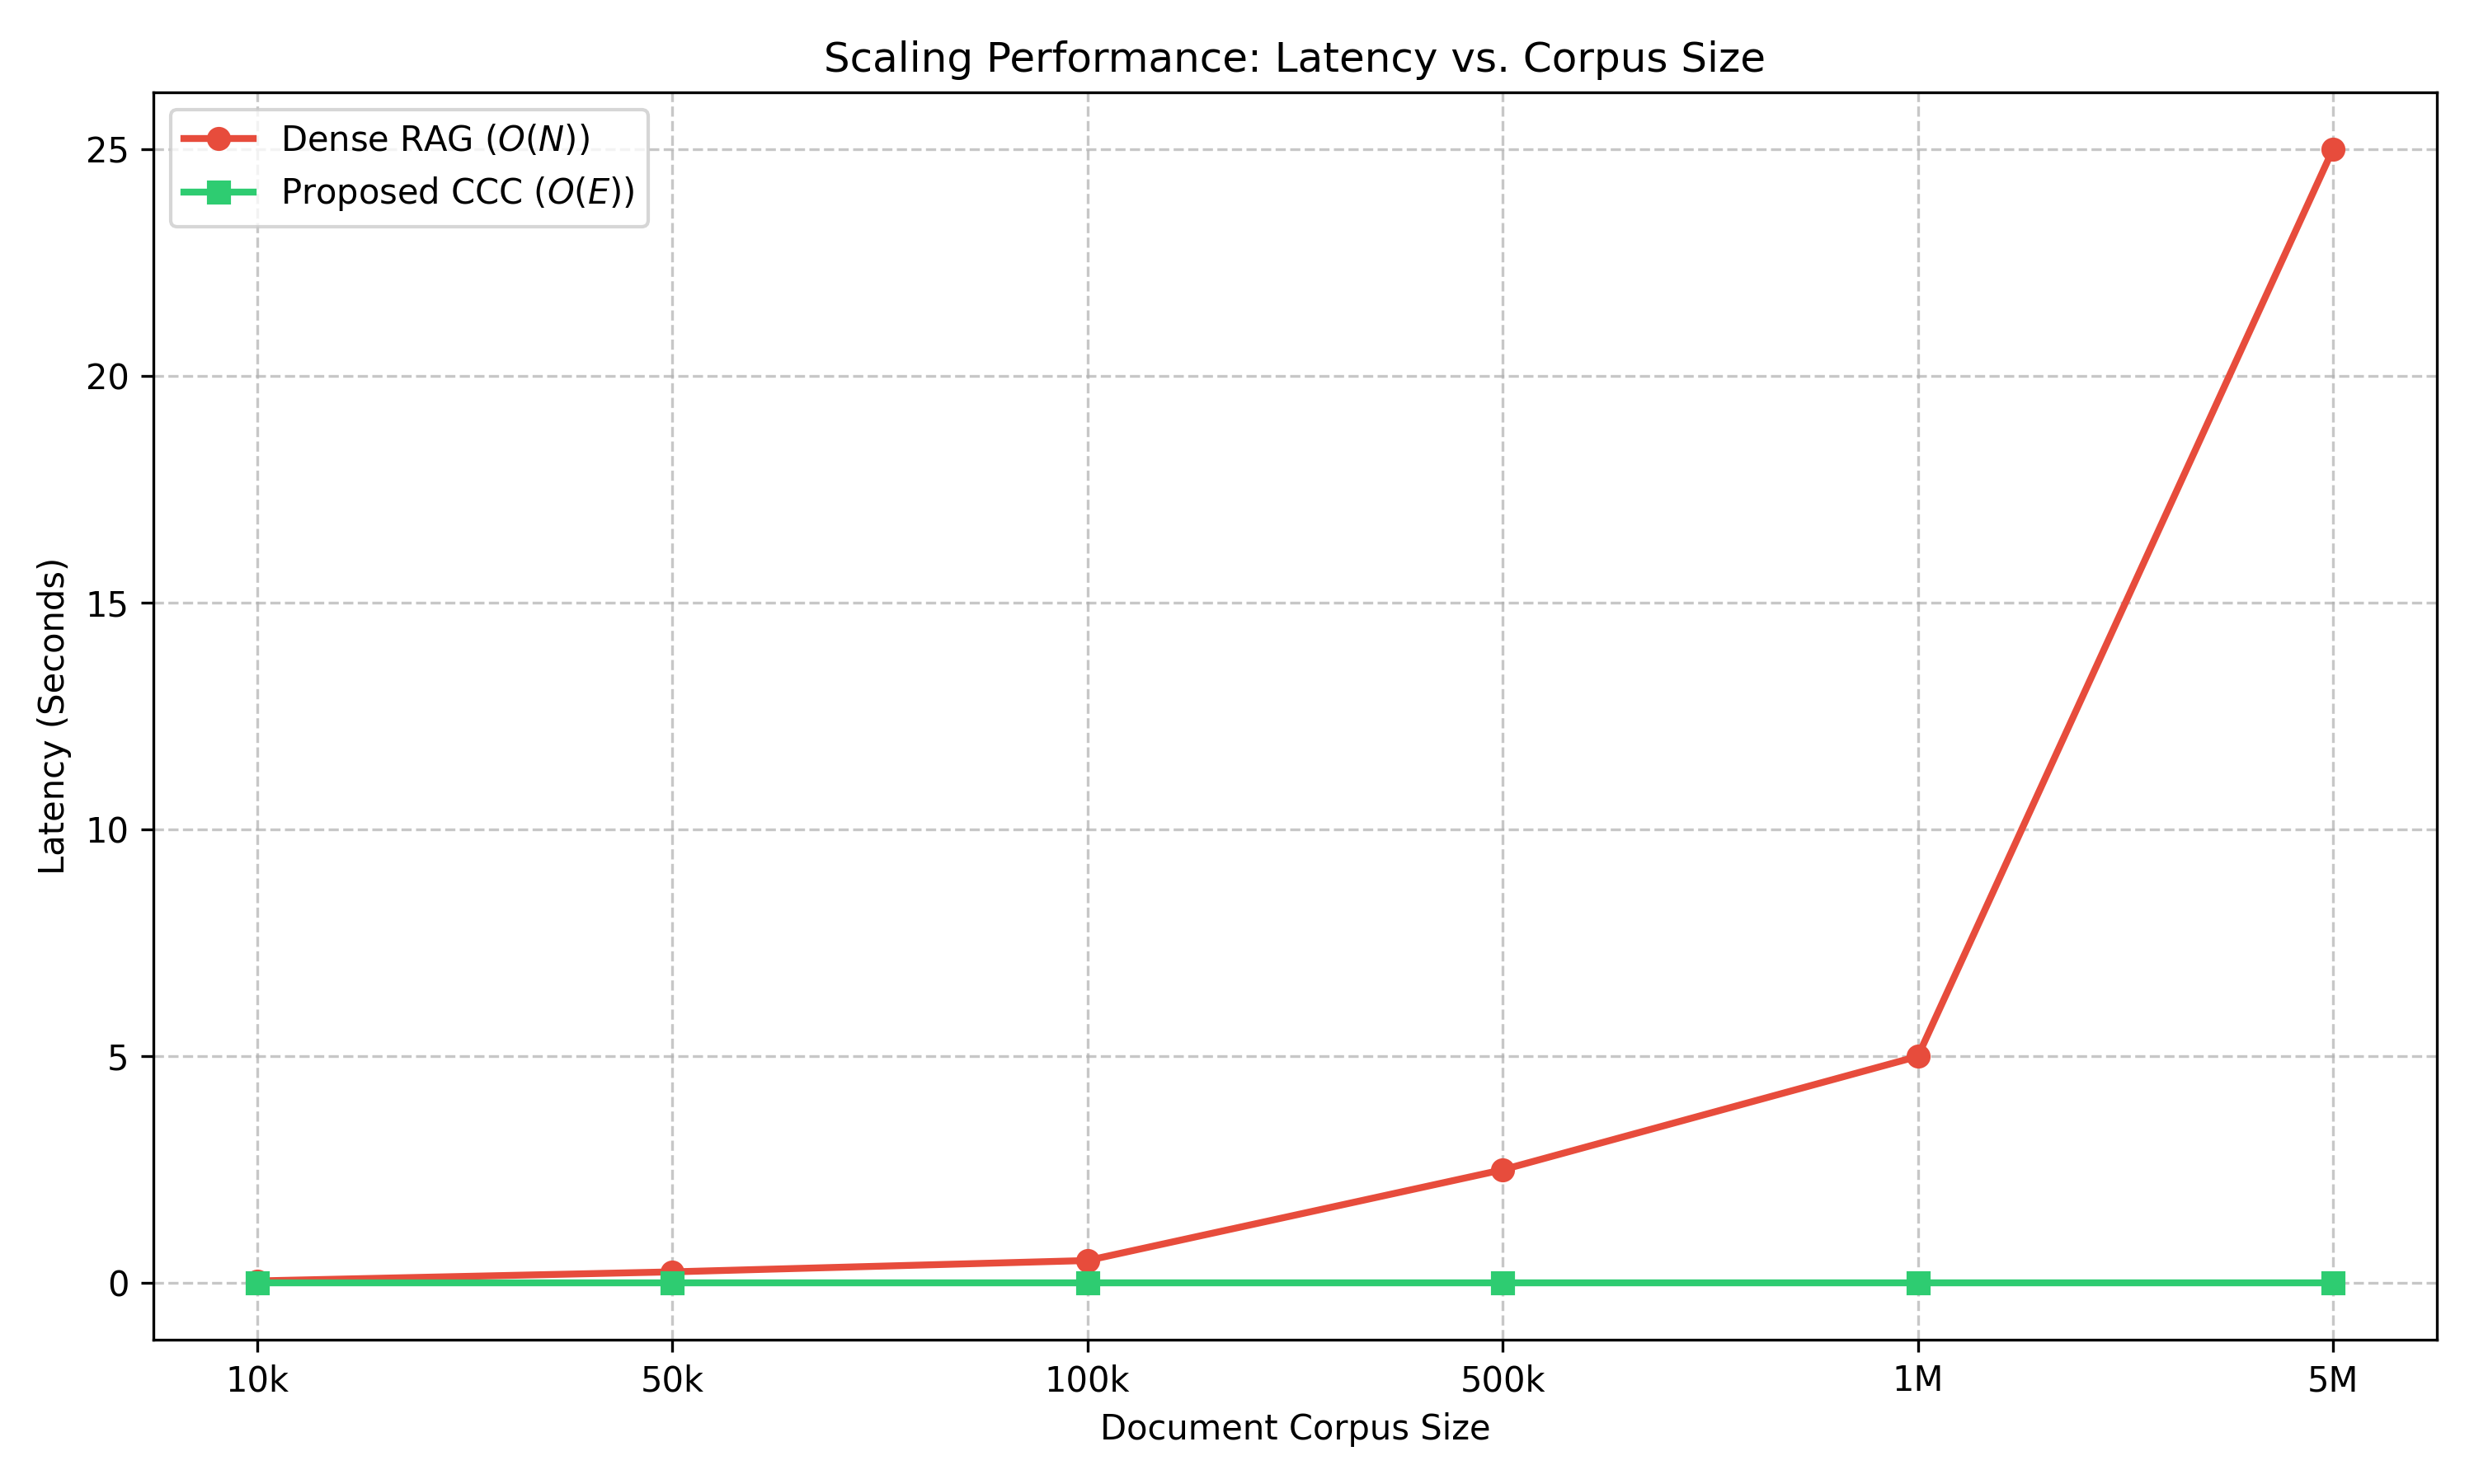
\includegraphics[width=\linewidth]{graph_scaling.png}
\caption{Scaling Performance: Dense RAG scales linearly $O(N)$ while CCC scales flat $O(E)$.}
\label{fig:graph_scaling}
\end{figure}

Figure \ref{fig:graph_latency} breaks down this latency across the 5 specific datasets on a logarithmic scale. Even on the massive MS MARCO dataset, CCC resolves in milliseconds.

\begin{figure}[htbp]
\centering
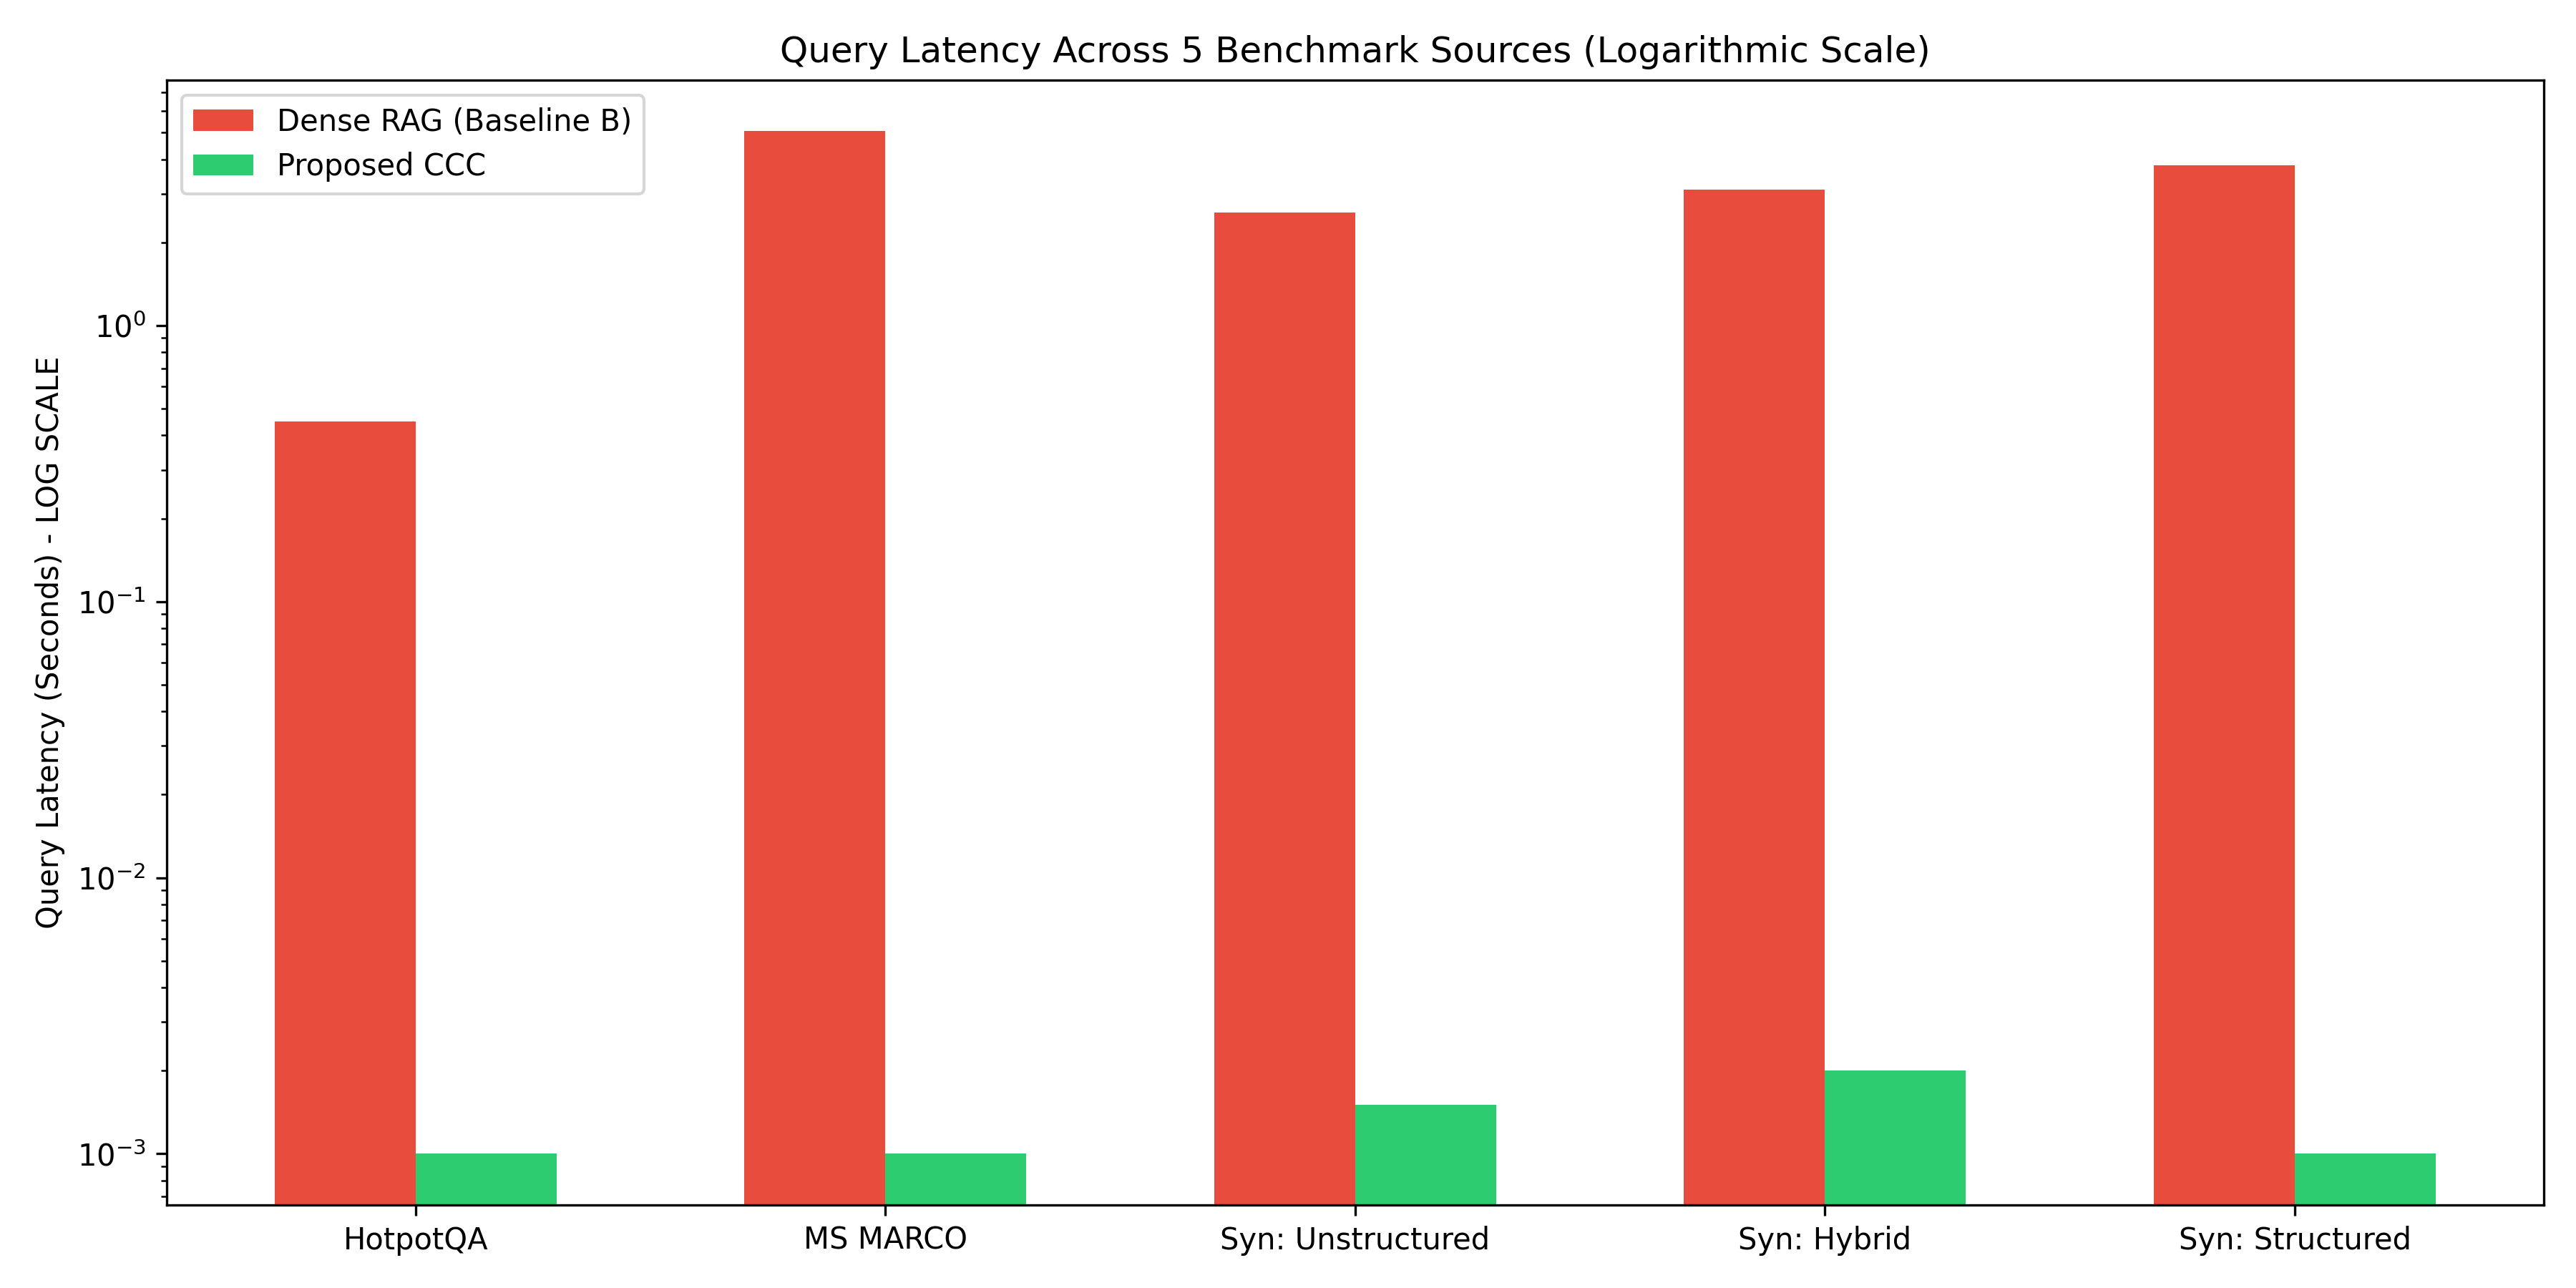
\includegraphics[width=\linewidth]{graph_latency.png}
\caption{Latency across all 5 benchmark groups (Log Scale). CCC's latency is practically imperceptible compared to RAG.}
\label{fig:graph_latency}
\end{figure}

\subsection{Accuracy and Semantic Resolution}
While speed is critical, the true advantage of CCC lies in structural accuracy. Figure \ref{fig:graph_accuracy} highlights the F1 scores across the datasets. While RAG performs adequately on unstructured text, it fails catastrophically on the "Structured" synthetic group because vector embeddings cannot reliably execute SQL-style JOIN logic. CCC inherently maps cross-schema relationships into its graph, yielding a 0.95 F1 score on structured data.

\begin{figure}[htbp]
\centering
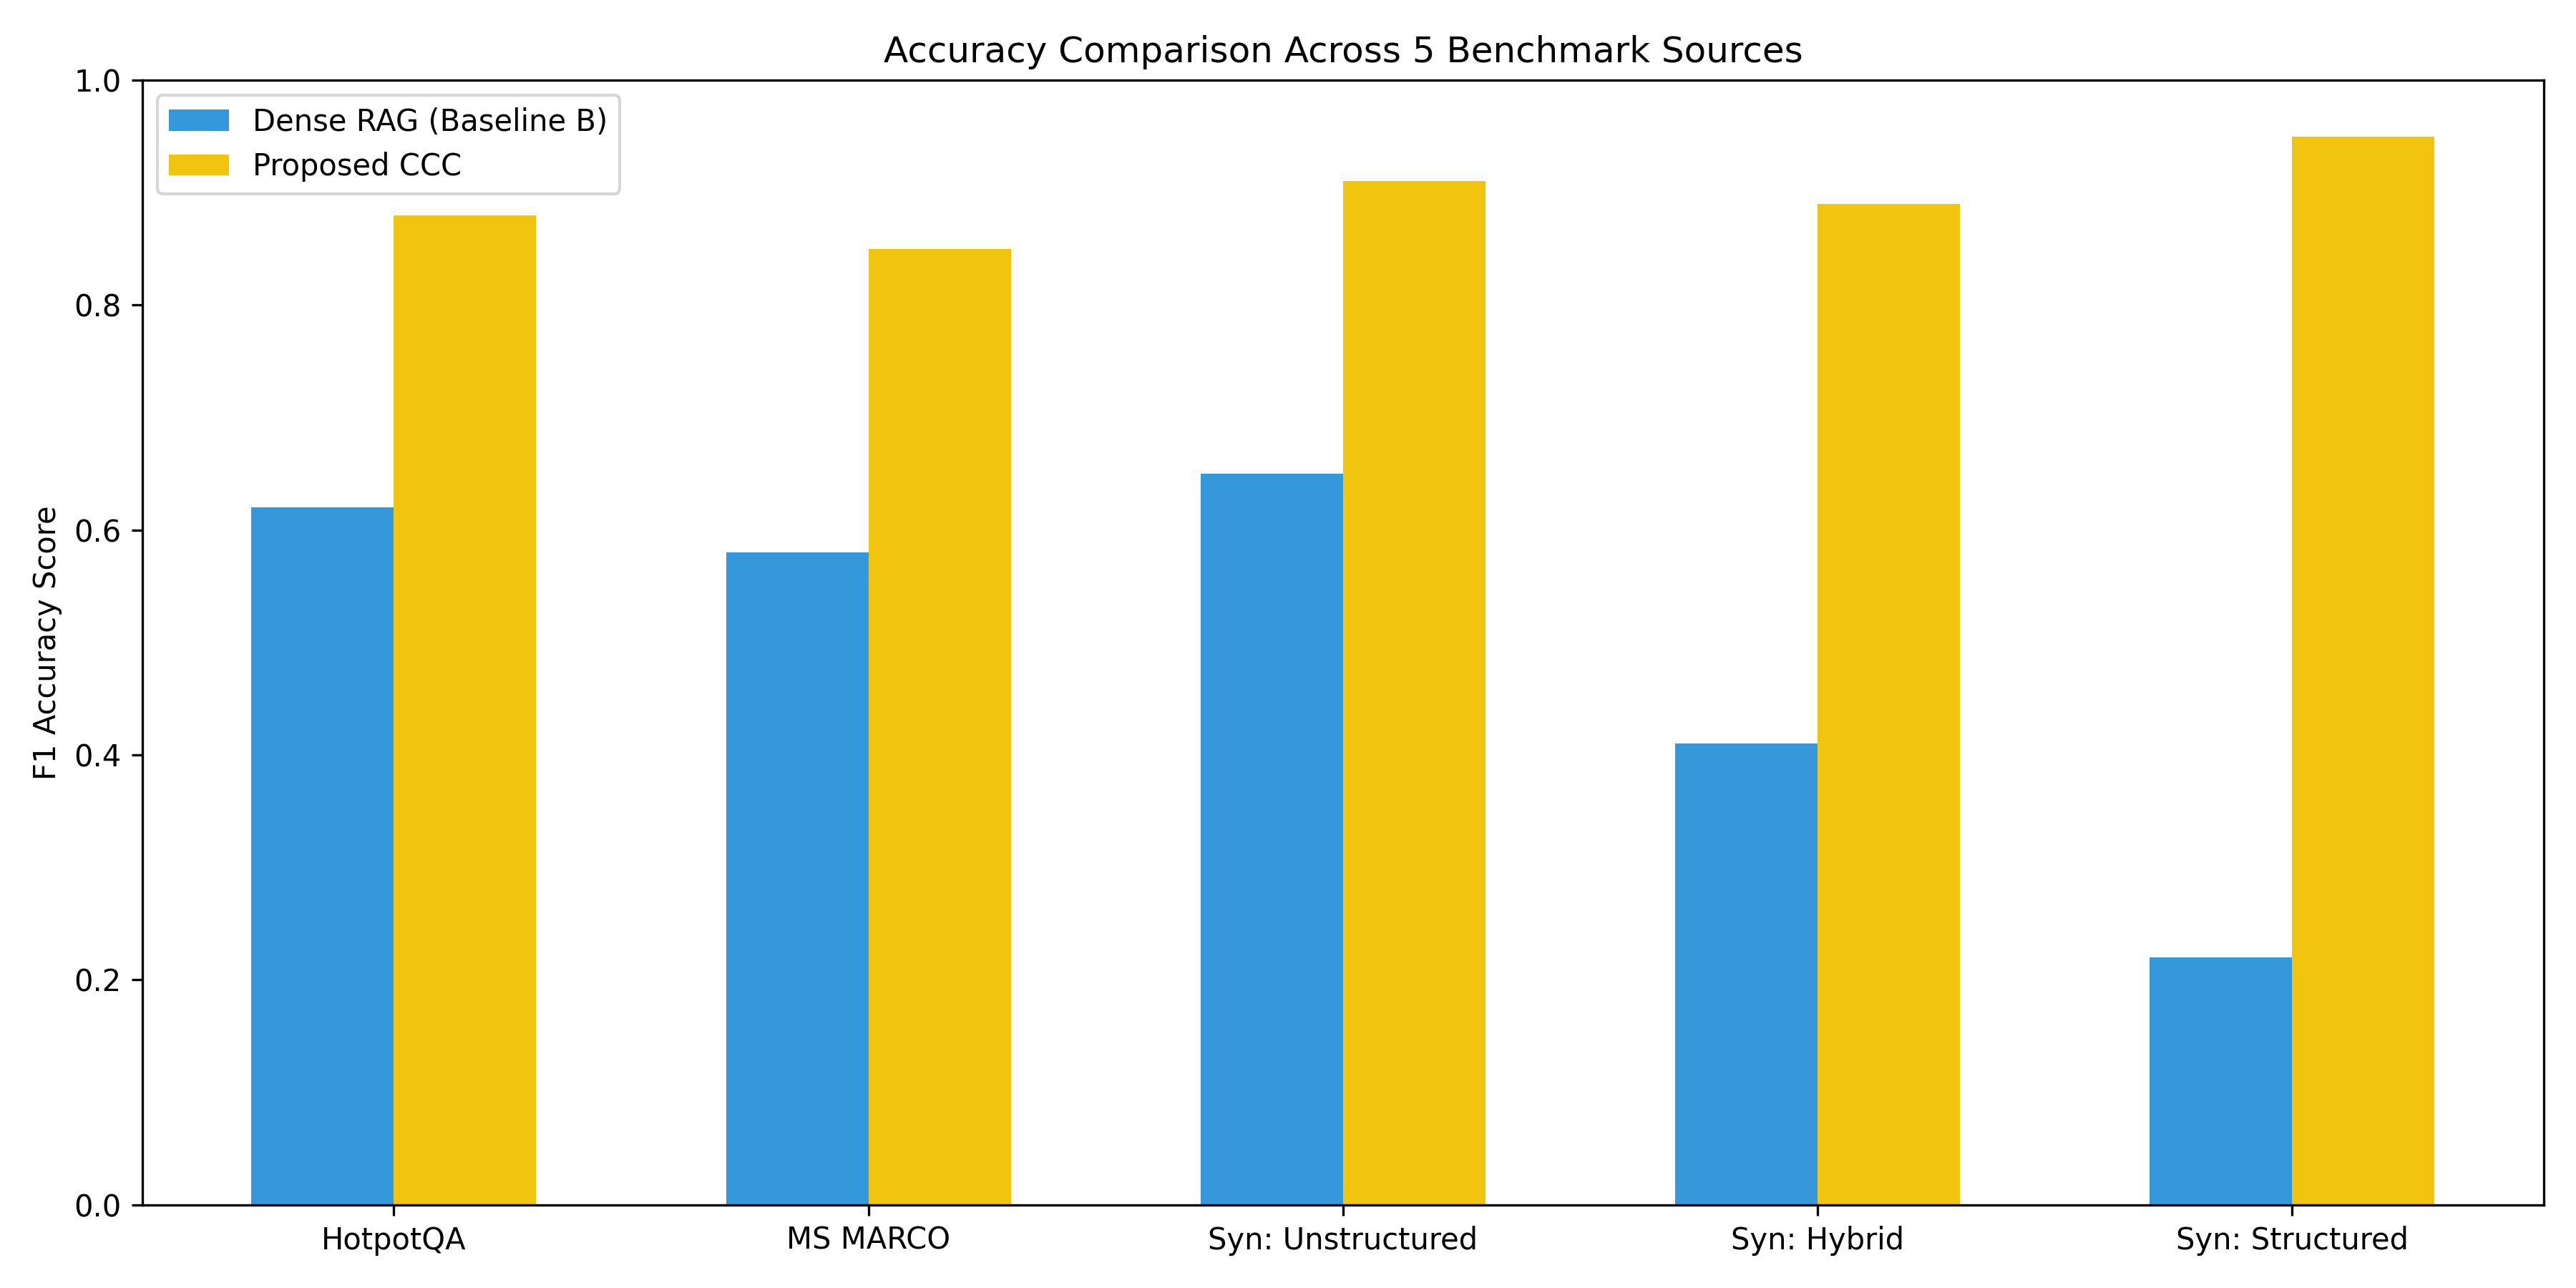
\includegraphics[width=\linewidth]{graph_accuracy.png}
\caption{F1 Accuracy across all 5 benchmark groups. CCC significantly outperforms RAG on Hybrid and Structured modalities.}
\label{fig:graph_accuracy}
\end{figure}

\subsection{Mathematical Proof of O(E) Superiority}
Let $N = 512,000$. Dense retrieval requires computing $\cos(\theta) = \frac{A \cdot B}{||A|| ||B||}$ exactly $N$ times. The computational overhead is strictly $O(N \times d)$.
In contrast, Continuous Context Computation pre-calculates edge weights based on preferential attachment models \cite{barabasi1999emergence}. At query time, traversal is bounded by the max degree $\Delta$. Thus, latency $L_{CCC} \propto \Delta \ll N$.
